\documentclass[11pt,openright,a4paper]{report}

 %%%%		Importation de tous les packages		%%%%%
\usepackage{tocloft}
\usepackage{graphicx}
\usepackage[utf8]{inputenc}
\usepackage[francais]{babel}
\usepackage{chngcntr}\counterwithout{footnote}{chapter} %permt de compter les notes de pieds de page
\usepackage{geometry}
\usepackage[T1]{fontenc}
\usepackage{sectsty}
\usepackage{fancyhdr}	% Permet de faire entête et pied de page
\usepackage{tabularx} 	% Pour faire des tableaux
\usepackage{hyperref}	% Pour faire les hyperliens internes
\usepackage{color}
\usepackage[svgnames]{xcolor}
\usepackage{tcolorbox}
\usepackage{tikz}
\usepackage{ifmtarg}
\usepackage{listings}
\usepackage{textcomp}
\usepackage{boxedminipage}
\usepackage[framemethod=default]{mdframed}
\usepackage{appendix}
\usepackage[
		%shortlop,
		under,
		side,
		%top,
		center,
		bottom,
	]{photo}
\usepackage{indentfirst}
\selectlanguage{francais}
%%%%%%%%%%%%%%%%%%%%%%%%%%%%%%%%%%%%%%%%%%%%%%%%%%%%%%


 %%%%	Gestion de la dimension du document		%%%%%
	\oddsidemargin 0.8cm
	\evensidemargin -0.2cm
	\textwidth 16cm
	\textheight 23cm
	\topmargin -0.5cm
%%%%%%%%%%%%%%%%%%%%%%%%%%%%%%%%%%%%%%%%%%%%%%%%%%%%%%


 %%%%	Préparation des nouvelles commandes		%%%%%
\renewcommand{\familydefault}{\sfdefault}

% Couleur et définition du thème chapter
\definecolor{monbleu}{HTML}{4E83A2}
\newcommand{\mychapter}[1]{\textcolor{monbleu}{\chapter{#1}}}

% Couleur et définition du thème section
\definecolor{monvert}{HTML}{0BA486}
\newcommand{\mysection}[1]{\textcolor{monvert}{\section{#1}}}

% Couleur et définition du thème subsection
\definecolor{monorange}{HTML}{E95D0F}
\newcommand{\mysubsection}[1]{\textcolor{monorange}{\subsection{#1}}}

% Définition D'Interlog Services
\newcommand{\interlog}{\textit{Interlog Services }}
%%%%%%%%%%%%%%%%%%%%%%%%%%%%%%%%%%%%%%%%%%%%%%%%%%%%%%%
			
			
			
%%%%		Pour mettre du code dans des boites		 %%%%%
\makeatletter				
	\newcommand{\mybox}[1]{%
  		\setbox0=\hbox{#1}%
  		\setlength{\@tempdima}{\dimexpr\wd0+13pt}%
  		\begin{tcolorbox}[	colframe=black!40,
  							boxrule=0.5pt,
  							arc=4pt,
      						left=6pt,
      						right=6pt,
      						top=6pt,
      						bottom=6pt,
      						boxsep=0pt,
      						width=16cm
      					]
    			#1
  		\end{tcolorbox}
}
\makeatother
%%%%%%%%%%%%%%%%%%%%%%%%%%%%%%%%%%%%%%%%%%%%%%%%%%%%%%%



%%%%		Pour coloriser les codes PHP ou autres		 %%%%%
\lstset{language=PHP,
    		basicstyle=\ttfamily\small,
    		breaklines=false,
    		prebreak=\raisebox{0ex}[0ex][0ex]{\ensuremath{\hookleftarrow}},
    		frame=lines,
    		showtabs=false,
    		showspaces=false,
    		showstringspaces=false,
    		keywordstyle=\color{red}\bfseries,
    		stringstyle=\color{green!50!black},
    		commentstyle=\color{gray}\itshape,
    		numbers=left,
    		captionpos=t,
    		escapeinside={\%*}{*)}
		}
%%%%%%%%%%%%%%%%%%%%%%%%%%%%%%%%%%%%%%%%%%%%%%%%%%%%%%%%%%%



%%%%%%%%		 	table of contents config			%%%%%%%%

\tocloftpagestyle{empty}
\setcounter{tocdepth}{1}
%%%%%%%%%%%%%%%%%%%%%%%%%%%%%%%%%%%%%%%%%%%%%%%%%%%%%%%%%



%%%%%%%%		 	Définition des entêtes et pieds de page			%%%%%%%%
\pagestyle{fancy}
	\lhead[\fancyplain{}{\raggedright\slshape\leftmark}]{}
	\chead{}
	\rhead[]{\fancyplain{}{\raggedleft\slshape\rightmark}}
	\fancyfoot[L]{Freddy Dubois}
	\rfoot[Licence Professionnelle - IUT Orléans]{Licence Professionnelle - IUT Orléans}
\fancypagestyle{plain} %Pour avoir le pied de page sur les première pages des chapitres
%%%%%%%%%%%%%%%%%%%%%%%%%%%%%%%%%%%%%%%%%%%%%%%%%%%%%%%%%%%%%%%%%%%%%%%%%

\begin{document}

%%%%%%%%%%		Page de garde		%%%%%%%%%%
	\begin{titlepage}
		\begin{Large}
		\baselineskip=7mm
		\noindent
			
\includegraphics[height=2cm]{./images/logo}
			\hfill
			
\includegraphics[height=2cm]{./images/logo_IUT}
			\vskip 30mm
			\begin{center}
				\rule{\textwidth}{1 mm}\\
				{\huge\sffamily\bfseries\baselineskip=1cm
					Développement d'application de PHP objet
				\par}
				\rule{\textwidth}{1 mm}\\
				{\Large\sffamily\bfseries 
					Rapport de stage de Licence professionnelle
				}
					\vskip 20mm
				Freddy DUBOIS
					\vskip 5mm
				17 février au 13 juin 2014
					\vskip 5mm
				Année universitaire 2013 - 2014
					\vfill
					\begin{photo}[!h]
						\centering
						\includegraphics[scale=1]{./images/siege_interlog}
					\end{photo}
					\vskip 5mm %45mm
				\begin{tabular}{l l p{4cm} l l}
					 Tuteur : Olivier ZOÏS		&	&	&	Tuteur : Enseignant	
				\end{tabular}
			\end{center}
		\end{Large}
	\end{titlepage}

%%%%%%%%%%%%%%%%%%%%%%%%%%%%%%%%%%%%%%%%%%%%%%%


%%%%%%%%%%%		Contenu du mémoire	%%%%%%%%%%
\cleardoublepage
\sloppy %permet d'éviter la césure des mots 
\section*{Remerciements}
\noindent
\phantomsection
\addcontentsline{toc}{section}{Remerciements}


Je tiens à remercier toute l'équipe informatique ainsi que M.Olivier ZOÏS mon maître de stage, directeur informatique 
au sein d'\interlog  pour m’avoir accepté en stage et de m’avoir
offert la possibilité d’une expérience professionnelle.\\


Je tiens également à remercier mon tuteur de stage et toute l’équipe enseignante qui
m’ont tous permis d’obtenir les connaissances nécessaires pour intégrer le milieu
professionnel.\\


Enfin, je remercie ma femme qui m’a soutenu tout au long de cette année universitaire
mais également dans mon projet de reconversion professionnelle.

\newpage



 % Mettre ici les remerciements

\tableofcontents			% Table des matières

\addcontentsline{toc}{chapter}{Table des mati\`eres}
\mychapter{Introduction}


Etudiant en Licence Professionnelle Réseaux Télécoms option Web et Mobile, 
j’ai réalisé un stage de seize semaines au sein d'\interlog à Orléans du 15 février au 7 juin 2014.\\

Durant mon stage, j’ai eu pour mission de développer des améliorations d'applications existantes
dans l'entreprise.\\


Dans un premier temps, je présenterai l’établissement qui m’a accueilli. L’exposition
des sujets de mon stage se fera dans un second temps, qui sera suivi par la présentation de
l’environnement de travail dans lequel les applications ont été développées. Une quatrième
partie sera consacrée au travail réalisé. Le bilan du stage conclura ce rapport.




\mychapter{Présentation}

%\begin{figure}[!h] % option !h pour dire que l'image sera à cet endroit
%	\centering
%	\includegraphics[scale=0.5]{../images/siege_interlog.jpg}
%	\caption{Siège social, Interlog Services à Orléans}
%	\label{Siege interlog}
%\end{figure}

\mysection{\interlog}

	\begin{photo}[!h]
		\centering
		\includegraphics[scale=0.5]{./images/siege_interlog.jpg}
		\caption{Siège social, \interlog à Orléans}
	\end{photo}

	\mysubsection{Présentation de l'entreprise}
		Anciennement \textit{ipseurope}, \interlog a été créé en 1999. Il s'agit de la première société à proposer sur le continent européen des audits de factures de transport.\\

		La société intervient au coeur de la \og Supply-Chain\fg \footnote{chaîne logistique}  et propose des prestations permettant des gains non négligeables. Les clients viennent de tous les secteurs d'activités (luxe, agroalimentaire, automobile \ldots).  \\

		Les équipes d'\interlog sont spécialisées dans la logistique et interviennent quotidiennement dans la gestion des opérations des clients. Elles interviennent sur:
		\begin{itemize}
			\item l'audit des factures transport,
			\item la gestion intégrée d’expéditions,
			\item l'organisation personnalisée du transport,
			\item le pilotage de plans de transport,
			\item l'approvisionnements mutualisés,
			\item le suivi et traçabilité des livraisons.
		\end{itemize}	
		
		\interlog  a su se développer à l'étranger. Elle est présente sur la France, l'Inde, les États-Unis et le Mexique.\\
		
		La société a pour but de réduire les coûts de transport des entreprises qui font appel a ses services.

    

    
    
    
   



\mysection{Organisation de l'entreprise}

\mysubsection{La direction}
	L'équipe de direction est composée :
	\begin{itemize}
		\item d'un président,
		\item d'une directrice générale et d'un directeur général,
		\item d'un directeur commercial,
		\item d'un directeur des opérations logistiques,
		\item d'un directeur informatique.
	\end{itemize}

\mysubsection{Le secteur informatique}
	Le secteur informatique est dirigé par le directeur informatique, Monsieur Zoïs. L'équipe de développeurs informatiques est composée de six personnes dont le chef de projets et  cinq développeurs.\\


\mysection{Matériel utilisé}

	\mysubsection{A Orléans}
		L'équipe de développement, constituée de cinq personnes, comprend cinq ordinateur montés sous Ubuntu 13.10.
		Les non développeurs sont équipés de 50 ordinateurs sous système OS Windows Seven.
		Sur trente serveurs que compte \interlog , le site d'Orléans en comprend neuf.

		

	\mysubsection{En Inde}
		L'équipe de développement est constitué de trois développeurs équipés également d'Ubuntu 13.10. Les non développeurs ont 100 ordinateurs équipés de Windows Seven.

		



\mychapter{Projet}


\mysection{Présentation du projet}
	Lors du stage, j'ai travaillé sur le projet Click \& Track . Il s'agit d'un portail Web développé en interne qui permet d'organiser les livraisons des clients en optimisant la communication entre les prestataires de transport et les logisticiens via un échange d'informations en temps réel qui couvre les fonctions suivantes:
	\begin{itemize}
		\item l'affectation des transporteurs,
		\item la transmission des ordres de transport,
		\item la gestion des plannings des entrepôts,
		\item le suivi des chargements et des livraisons,
		\item la gestion des litiges et demandes d'émargés,
		\item le contrôle de la facturation transport,
		\item les indicateurs de qualités / Kpi's. \footnote{Key Performance Indicators, indicateurs mesurables d'aide décisionnelles}
	\end{itemize}
	


\mysection{Autour du projet}


\mychapter{Codage}


\mysection{Rêgles de codage}


\mysubsection{Identifiers}

Noms des classes : 

Noms des fonctions :

Noms des variables :




\mysection{Documentation du code}


\mybox{
%\begin{boxedminipage}[poslb]{15.5cm}
\lstinputlisting[caption={Un hello world},
  				label=hello,
  				tabsize=2,
  				%backgroundcolor=yellow,
  				language=PHP]{./code/hello.php}
%\end{boxedminipage}
}
comme le montre \ref{hello}
%\begin{lstlisting}[language=PHP]
%\lstinputlisting{hello.php}
%\end{lstlisting}




\mychapter{Bilan}


\mysection{Bilan personnel}
	


\mysection{Bilan en entreprise}


%
\mychapter{Annexes}


\mysection{Mes annexes}
	




\addcontentsline{toc}{chapter}{Annexes}
%%%%%%%%%%%%%%%%%%%%%%%%%%%%%%%%%%%%%%%%%%%%%%%

\end{document}
